\documentclass[aspectratio=169,11pt]{beamer}

\usetheme[progressbar=frametitle,numbering=fraction,block=fill]{metropolis}
\usepackage[T1]{fontenc}
\usepackage[scaled=0.95]{helvet}
\renewcommand{\familydefault}{\sfdefault}
\usepackage{amsmath}
\usepackage{graphicx}
\usepackage{booktabs}
\usepackage{multicol}
\usepackage{tikz}
\usetikzlibrary{arrows.meta,positioning}
\usepackage[round]{natbib}
\usepackage{url}

\graphicspath{{../figures/}}
% Generated by scripts/11_slide_numbers.py. Do not edit.
\newcommand{\nNHighAll}{5}
\newcommand{\nNHighWindow}{4}
\newcommand{\nMaxSpacing}{3.8}
\newcommand{\nNSamples}{1362}
\newcommand{\nNBins}{527}
\newcommand{\nSpan}{2{,}630}
\newcommand{\nNativePeak}{3.87}
\newcommand{\nEventLevel}{3.43}
\newcommand{\nSecondPeak}{2.12}
\newcommand{\nMargin}{1.3}
\newcommand{\nZscore}{5.1}
\newcommand{\nKurtAll}{1.23}
\newcommand{\nKurtEx}{0.21}
\newcommand{\nMedEOne}{-0.45}
\newcommand{\nMedETwo}{0.12}
\newcommand{\nMedEThree}{-0.78}
\newcommand{\nTauNative}{11.5}
\newcommand{\nTauBinned}{19.5}
\newcommand{\nPettittYear}{1355}
\newcommand{\nMKp}{0.46}
\newcommand{\nNRuns}{26}
\newcommand{\nSpellStart}{475}
\newcommand{\nSpellEnd}{545}
\newcommand{\nSpellDur}{70}
\newcommand{\nRankSeverity}{2}
\newcommand{\nRankDuration}{2}
\newcommand{\nRankIntensity}{3}
\newcommand{\nWorstStart}{730}
\newcommand{\nWorstEnd}{935}
\newcommand{\nThreshold}{0.76}
\newcommand{\nNPeaks}{19}
\newcommand{\nRatePerCentury}{0.72}
\newcommand{\nXi}{-0.12}
\newcommand{\nXiLo}{-1.61}
\newcommand{\nXiHi}{0.21}
\newcommand{\nTMLE}{11{,}594}
\newcommand{\nTBootLo}{3{,}196}
\newcommand{\nTBootInf}{34}
\newcommand{\nTEmcee}{4{,}035}
\newcommand{\nPRecord}{20}
\newcommand{\nRLThousand}{2.13}
\newcommand{\nXiFifty}{0.02}
\newcommand{\nXiHundred}{-0.04}
\newcommand{\nTFifty}{5{,}897}
\newcommand{\nTHundred}{9{,}767}
\newcommand{\nXiWithout}{-0.86}
\newcommand{\nEndWithout}{2.13}
\newcommand{\nTMSWith}{4{,}374}
\newcommand{\nTMSWithout}{9{,}138}
\newcommand{\nTMSWithoutHi}{532{,}812}
\newcommand{\nTUniWith}{4{,}986}
\newcommand{\nUniInf}{60}
\newcommand{\nPRecMSWith}{46}
\newcommand{\nPRecMSWithout}{29}
\newcommand{\nPRecUniWith}{42}
\newcommand{\nPRecUniWithout}{8}
\newcommand{\nBgEvent}{+0.19}
\newcommand{\nResid}{3.24}
\newcommand{\nTResid}{13{,}041}
\newcommand{\nTNS}{3{,}791}
\newcommand{\nGridMin}{5{,}562}
\newcommand{\nGridMax}{20{,}766}
\newcommand{\nGridCells}{36}
\newcommand{\nGridInf}{19}
\newcommand{\nMuFifty}{0.08}
\newcommand{\nSigmaFifty}{0.67}
\newcommand{\nNFifty}{53}
\newcommand{\nXiLoFifty}{-0.21}
\newcommand{\nXiHiFifty}{0.16}
\newcommand{\nTBootLoFifty}{2{,}087}
\newcommand{\nTBootMedFifty}{6{,}974}
\newcommand{\nTBootInfFifty}{4}
\newcommand{\nRLThousandFifty}{2.14}
\newcommand{\nRLThousandLoFifty}{1.59}
\newcommand{\nRLThousandHiFifty}{2.65}
\newcommand{\nRLFiveHundredFifty}{1.63}
\newcommand{\nRLTenKFifty}{3.82}
\newcommand{\nXiWithoutFifty}{-0.11}
\newcommand{\nTWithoutFifty}{54{,}812}
\newcommand{\nPRecFifty}{36}
\newcommand{\nMuHundred}{0.42}
\newcommand{\nSigmaHundred}{0.72}
\newcommand{\nNHundred}{27}
\newcommand{\nXiLoHundred}{-0.52}
\newcommand{\nXiHiHundred}{0.68}
\newcommand{\nTBootLoHundred}{1{,}549}
\newcommand{\nTBootMedHundred}{8{,}808}
\newcommand{\nTBootInfHundred}{19}
\newcommand{\nRLThousandHundred}{1.97}
\newcommand{\nRLThousandLoHundred}{1.39}
\newcommand{\nRLThousandHiHundred}{2.57}
\newcommand{\nRLFiveHundredHundred}{1.46}
\newcommand{\nRLTenKHundred}{3.44}
\newcommand{\nXiWithoutHundred}{-0.31}
\newcommand{\nTWithoutHundred}{$\infty$}
\newcommand{\nPRecHundred}{24}
\newcommand{\nRhoFifty}{0.01}
\newcommand{\nRhoHundred}{$<$\,0.001}


\definecolor{okblue}{HTML}{0072B2}
\definecolor{okverm}{HTML}{D55E00}
\definecolor{okgreen}{HTML}{009E73}
\definecolor{okorange}{HTML}{E69F00}
\definecolor{inkgrey}{HTML}{4D4D4D}
\setbeamercolor{alerted text}{fg=okverm}
\setbeamercolor{progress bar}{fg=okblue,bg=okblue!15}
\setbeamercolor{frametitle}{bg=black!85,fg=white}
\setbeamercolor{block title}{bg=okblue!15,fg=black}
\setbeamercolor{block body}{bg=okblue!5,fg=black}
\setlength{\bibsep}{1.5pt}

\newcommand{\permil}{\ensuremath{\text{\textperthousand}}}
\newcommand{\dO}{$\delta^{18}$O}
\newcommand{\figh}{0.60\textheight}

\title{Quantifying the sixth-century Arabian drought}
\subtitle{Extreme value analysis of the Hoti Cave H12 stalagmite \dO{}
  record}
\author{Sandy Hardian Susanto Herho \quad {\small(NIM 32426003)}}
\institute{Weather and Climate Extremes\\
  Doctoral Program in Earth Sciences, Bandung Institute of Technology}
\date{October 2026\\[0.6em]
  {\footnotesize Code and data:
  \url{https://github.com/sandyherho/utsCuacaIklimEks}}}

\begin{document}

% =================================================================== 1
\maketitle

% =================================================================== 2
\begin{frame}{The claim under test}
  \begin{columns}[T]
    \begin{column}{0.55\textwidth}\small
      \cite{Fleitmann2022} combine a new stalagmite record from northern
      Oman with regional proxies and history.
      \begin{itemize}\setlength{\itemsep}{2pt}
        \item Himyar dominated southern Arabia until the Aksumite conquest
              of 525 CE and dissolved during the sixth century.
        \item The stalagmite shows its most severe aridity at about
              500--530 CE, peaking near 523 $\pm$ 30 CE.
        \item The drought, the authors argue, eroded the resilience of an
              economy built on rain-fed and runoff agriculture.
      \end{itemize}
    \end{column}
    \begin{column}{0.42\textwidth}
      \begin{block}{Aim}
        \small Using only the \dO{} series and extreme value statistics,
        quantify
        \begin{enumerate}
          \item how large the drought was,
          \item how rare it was,
          \item whether the signal and its rarity are physically and
                statistically credible.
        \end{enumerate}
      \end{block}
    \end{column}
  \end{columns}
\end{frame}

% =================================================================== 3
\begin{frame}{The archive: stalagmite H12 from Hoti Cave}
  \begin{columns}[T]
    \begin{column}{0.56\textwidth}\small
      \begin{itemize}\setlength{\itemsep}{3pt}
        \item Hoti Cave, northern Oman (23\textdegree05$'$N,
              57\textdegree21$'$E, 800 m). Annual rainfall 50--255 mm,
              about two thirds of it in winter and spring from Mediterranean
              frontal systems \citep{Fleitmann2022}.
        \item Rain seeps through soil and limestone, reaches the cave as
              drip water, and deposits calcite layer by layer. The
              stalagmite grew about 0.23 mm per year.
        \item Ages come from 20 uranium-thorium dates; the isotope samples
              have a resolution of about 2 years.
      \end{itemize}
    \end{column}
    \begin{column}{0.40\textwidth}
      \begin{block}{What we can and cannot read}
        \small Calcite stores the oxygen isotope ratio of the drip water,
        which carries the rainfall signal. It does not record rainfall in
        millimeters directly; the link must be calibrated.
      \end{block}
    \end{column}
  \end{columns}
\end{frame}

% =================================================================== 4
\begin{frame}{What \dO{} measures}
  \begin{columns}[T]
    \begin{column}{0.52\textwidth}\small
      Oxygen has a light isotope ($^{16}$O) and a rare heavy one ($^{18}$O).
      With $R = {}^{18}\mathrm{O}/{}^{16}\mathrm{O}$,
      \[
        \delta^{18}\mathrm{O} =
        \left(\frac{R_\mathrm{sample}}{R_\mathrm{standard}} - 1\right)
        \times 1000 \quad (\text{\permil}).
      \]
      Here the standard is VPDB. A more negative value means relatively
      less $^{18}$O.
      \par\medskip
      Heavy water molecules condense more readily, so rain is enriched in
      $^{18}$O relative to the vapor it leaves behind
      \citep{Dansgaard1964}.
    \end{column}
    \begin{column}{0.45\textwidth}
      \begin{block}{Rayleigh distillation}
        \small As a fraction $f$ of the original vapor remains,
        \[
          \delta_\mathrm{v} \approx \delta_{\mathrm{v},0}
          + 1000\,(\alpha - 1)\ln f ,
        \]
        with $\alpha \approx 1.0098$ (liquid--vapor, 20\,\textdegree C).
        Raining out half of the vapor ($f=0.5$) lowers the vapor, and the
        rain that follows, by about 7\permil.
      \end{block}
    \end{column}
  \end{columns}
\end{frame}

% =================================================================== 5
\begin{frame}{The amount effect: why higher \dO{} means less rain}
  \centering
  \begin{tikzpicture}[
      box/.style={draw=okblue, fill=okblue!8, rounded corners=2pt,
        text width=25mm, minimum height=12mm, align=center,
        font=\scriptsize},
      wet/.style={box, text width=31mm, fill=okblue!18},
      dry/.style={box, text width=31mm, draw=okverm, fill=okverm!10},
      arr/.style={-{Stealth[length=2mm]}, thick, inkgrey}]
    \node[box] (src) {Moist air from the Mediterranean and Arabian Sea};
    \node[wet, right=7mm of src, yshift=8.5mm] (w)
      {\textbf{Wet season:} intense rain removes much vapor; rain has
       low \dO{}};
    \node[dry, right=7mm of src, yshift=-8.5mm] (d)
      {\textbf{Dry season:} weak rain; drops and soil water evaporate;
       high \dO{}};
    \node[box, right=7mm of w, yshift=-8.5mm] (k)
      {Soil and karst mix rain over months to years};
    \node[box, right=7mm of k, text width=21mm] (c)
      {Calcite \dO{} records the drip water};
    \draw[arr] (src) -- (w); \draw[arr] (src) -- (d);
    \draw[arr] (w) -- (k); \draw[arr] (d) -- (k); \draw[arr] (k) -- (c);
  \end{tikzpicture}
  \par\medskip
  \begin{itemize}\small\setlength{\itemsep}{2pt}
    \item In the tropics and subtropics, rain \dO{} falls as rain amount
          rises: the \alert{amount effect} \citep{Dansgaard1964,Lachniet2009}.
    \item At Hoti it is calibrated: H12 \dO{} correlates with instrumental
          Oman rainfall at $r = -0.69$ \citep{Fleitmann2022}.
  \end{itemize}
\end{frame}

% =================================================================== 6
\begin{frame}{At Hoti, dry years push \dO{} up through three processes}
  \centering\footnotesize
  \begin{tabular}{@{}p{0.22\textwidth}p{0.44\textwidth}p{0.22\textwidth}@{}}
    \toprule
    Process & Mechanism & Dry-year effect \\
    \midrule
    Amount effect & Less rainout; falling drops evaporate & \dO{} higher \\
    Soil evaporation & Light rain on dry soil is enriched before it
      infiltrates & \dO{} higher \\
    Cave kinetics & Slow drips degas CO$_2$ fast; calcite forms out of
      isotopic equilibrium & \dO{} higher \\
    \bottomrule
  \end{tabular}
  \par\medskip
  \begin{itemize}\footnotesize\setlength{\itemsep}{2pt}
    \item Kinetic effects at Hoti are confirmed by the strong coupling of
          \dO{} and $\delta^{13}$C ($r^2=0.52$) \citep{Fleitmann2022}.
          Because all three act in the same direction, dry extremes are
          \alert{amplified}: \dO{} responds nonlinearly to rainfall.
    \item Temperature is a minor control. Calcite \dO{} changes by about
          $-0.2$\permil{} per \textdegree C \citep{Lachniet2009}; a
          $+3.4$\permil{} excursion would need more than 15\,\textdegree C
          of cave cooling. This study therefore measures how extreme the
          \emph{proxy} is, not rainfall in millimeters.
  \end{itemize}
\end{frame}

% =================================================================== 7
\begin{frame}{The record: one excursion stands out}
  \centering
  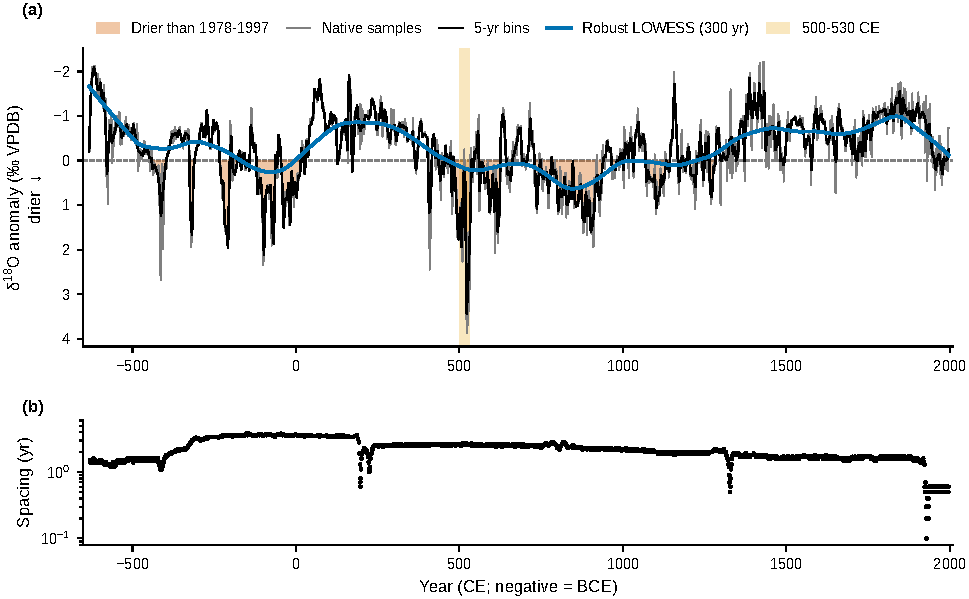
\includegraphics[width=\textwidth,height=0.52\textheight,keepaspectratio]{fig01_record_overview}
  \par\vspace{-0.3em}
  \begin{itemize}\footnotesize\setlength{\itemsep}{1pt}
    \item \textbf{Reading the figure.} (a) Drought plots \emph{downward}.
          Grey: raw samples; black: 5-yr means; blue: smooth 300-yr trend;
          orange shading: drier than 1978--1997. The yellow band marks
          500--530 CE.
    \item (b) Time between samples, from 0.1 to \nMaxSpacing{} yr. Raw
          samples therefore average very different spans of time, which the
          next step corrects.
  \end{itemize}
\end{frame}

% =================================================================== 8
\begin{frame}{Step 1. Put all samples on an even time step}
  \begin{columns}[T]
    \begin{column}{0.53\textwidth}\small
      \textbf{Problem.} The samples are evenly spaced along the
      stalagmite, not in time. A sample that covers 3 years blends a dry
      year with wetter ones; a sample that covers half a year does not.
      Extremes would look larger where sampling is fine.
      \par\medskip
      \textbf{Method.} Cut the timeline into 5-yr boxes and average the
      $n_k$ samples in box $k$:
      \[
        \bar{x}_k = \frac{1}{n_k}\sum_{i \in k} x_i .
      \]
      Five years exceeds the widest gap (\nMaxSpacing{} yr), so every box
      holds at least one real measurement and nothing is invented.
    \end{column}
    \begin{column}{0.43\textwidth}
      \begin{block}{Result}
        \small
        \begin{itemize}\setlength{\itemsep}{2pt}
          \item \nNBins{} evenly spaced values, each representing 5 years.
          \item Driest value: $+\nEventLevel$\permil{} at 520--525 CE.
          \item It lies \alert{\nZscore{} standard deviations} above the
                mean of the rest of the record.
        \end{itemize}
      \end{block}
    \end{column}
  \end{columns}
\end{frame}

% =================================================================== 9
\begin{frame}{Why a special theory for extremes}
  \begin{columns}[T]
    \begin{column}{0.52\textwidth}\small
      \begin{itemize}\setlength{\itemsep}{3pt}
        \item Ordinary statistics describe the typical year. A drought study
              is about the rare years in the tail, where a bell-curve
              (normal) fit is usually wrong.
        \item Extreme value theory does for extremes what the central limit
              theorem does for averages: the largest values follow a small
              family of curves, whatever the shape of the full data
              \citep{Coles2001}.
        \item It turns ``this value is very large'' into ``a value this
              large happens, on average, once every $T$ years''.
      \end{itemize}
    \end{column}
    \begin{column}{0.44\textwidth}
      \begin{block}{The idea of block maxima}
        \small Hydrologists design dams from the \emph{largest flood of
        each year}. We do the same with time blocks: keep only the driest
        value of each block, then study how those driest values are
        distributed.
        \par\smallskip
        Here a year is too short, so the blocks are 50 years (main) and
        100 years (check).
      \end{block}
    \end{column}
  \end{columns}
\end{frame}

% =================================================================== 10
\begin{frame}{Step 2. Cut the record into blocks}
  \begin{columns}[T]
    \begin{column}{0.53\textwidth}\small
      \textbf{Method.} Split the 5-yr series into blocks of length $B$ and
      keep the driest value of each block $j$:
      \[
        M_j = \max\{\bar{x}_k : k \in \text{block } j\},
        \qquad j = 1, \dots, m .
      \]
      $B = 50$ yr gives $m = \nNFifty$ maxima; $B = 100$ yr gives
      $m = \nNHundred$.
      \par\medskip
      \textbf{Trade-off.} Longer blocks hold truer extremes but give fewer
      of them; shorter blocks give more maxima, some of which are not very
      extreme.
    \end{column}
    \begin{column}{0.43\textwidth}
      \begin{block}{Independence of the blocks}
        \small The theory needs maxima that do not influence each other.
        Dry and wet spells carry a memory that fades as
        \[
          \rho(\Delta t) = e^{-\Delta t/\tau},
        \]
        with $\tau \approx \nTauNative$ yr in this record
        \citep{Mudelsee2002}. Between blocks 50 yr apart,
        $\rho \approx \nRhoFifty$; at 100 yr, $\rho$ \nRhoHundred.
        \alert{Neighboring blocks are practically independent.}
      \end{block}
    \end{column}
  \end{columns}
\end{frame}

% =================================================================== 11
\begin{frame}{Step 3. The generalized extreme value (GEV) distribution}
  \begin{columns}[T]
    \begin{column}{0.53\textwidth}\footnotesize
      Block maxima follow one curve, the GEV \citep{Coles2001}. The chance
      that a block maximum stays \emph{below} a level $z$ is
      \[
        G(z) = \exp\!\left\{-\left[1 + \xi\,\frac{z-\mu}{\sigma}
        \right]^{-1/\xi}\right\},
      \]
      valid where $1 + \xi (z-\mu)/\sigma > 0$. When $\xi = 0$ it becomes
      the Gumbel curve
      \[
        G(z) = \exp\!\left\{-\exp\!\left[-\frac{z-\mu}{\sigma}\right]
        \right\}.
      \]
      The chance of \emph{exceeding} $z$ in one block is $1 - G(z)$.
    \end{column}
    \begin{column}{0.43\textwidth}
      \begin{block}{Three numbers, in plain words}
        \footnotesize\textbf{Location $\mu$:} the typical driest value of a block.
        \par\smallskip
        \textbf{Scale $\sigma$:} how much block maxima vary around $\mu$.
        \par\smallskip
        \textbf{Shape $\xi$:} how fast very dry blocks become rare.
        \begin{itemize}\setlength{\itemsep}{1pt}
          \item $\xi<0$: a ceiling exists at $\mu - \sigma/\xi$.
          \item $\xi=0$: each extra unit of dryness cuts the chance by the
                same factor.
          \item $\xi>0$: no ceiling.
        \end{itemize}
      \end{block}
    \end{column}
  \end{columns}
\end{frame}

% =================================================================== 12
\begin{frame}{The block maxima method in one picture}
  \centering
  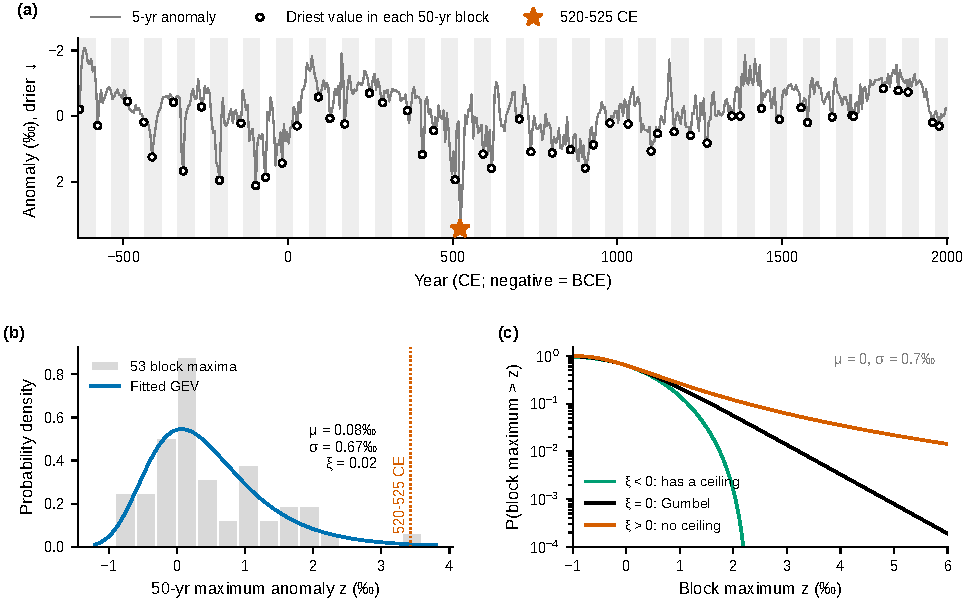
\includegraphics[width=\textwidth,height=0.56\textheight,keepaspectratio]{fig14_bm_method}
  \par\vspace{-0.3em}
  \begin{itemize}\footnotesize\setlength{\itemsep}{1pt}
    \item \textbf{Reading the figure.} (a) Grey and white stripes: 50-yr
          blocks. Circles: the driest value of each block; star: 520--525 CE.
          (b) Histogram of the \nNFifty{} block maxima and the fitted GEV
          curve; the event sits alone at the far right. (c) How the shape
          $\xi$ changes the chance of a very dry block.
  \end{itemize}
\end{frame}

% =================================================================== 13
\begin{frame}{Step 4. Fitting the curve and measuring uncertainty}
  \begin{columns}[T]
    \begin{column}{0.53\textwidth}\footnotesize
      \textbf{Maximum likelihood.} Choose $\mu, \sigma, \xi$ that make the
      $m$ observed maxima $z_1, \dots, z_m$ most probable, by maximizing
      the log-likelihood \citep{Coles2001}
      \[
        \begin{aligned}
          \ell(\mu,\sigma,\xi) = &-m\ln\sigma
            - \left(1 + \tfrac{1}{\xi}\right)\sum_{j=1}^{m}
              \ln\!\left[1 + \xi\,\tfrac{z_j-\mu}{\sigma}\right] \\
          &- \sum_{j=1}^{m}
              \left[1 + \xi\,\tfrac{z_j-\mu}{\sigma}\right]^{-1/\xi}.
        \end{aligned}
      \]
      In words: try many curves and keep the one under which our data are
      least surprising (Python \texttt{pyextremes}).
    \end{column}
    \begin{column}{0.43\textwidth}
      \begin{block}{Bootstrap uncertainty}
        \footnotesize Nature gave us one set of block maxima; a slightly different
        history would give a slightly different set. The bootstrap imitates
        this \citep{Efron1979}:
        \begin{enumerate}\setlength{\itemsep}{1pt}
          \item draw $m$ maxima at random, with replacement;
          \item refit the GEV;
          \item repeat thousands of times.
        \end{enumerate}
        The spread of the refitted answers is the uncertainty. We report
        the 5--95\,\% range.
      \end{block}
    \end{column}
  \end{columns}
\end{frame}

% =================================================================== 14
\begin{frame}{Step 5. From the curve to return levels and return periods}
  \begin{columns}[T]
    \begin{column}{0.53\textwidth}\small
      \textbf{Return period} of a level $z$, in years:
      \[
        T(z) = \frac{B}{1 - G(z)} .
      \]
      \textbf{Return level}: the dryness reached once every $T$ years,
      \[
        z_T = \mu - \frac{\sigma}{\xi}\left[1 - y_T^{-\xi}\right],
        \qquad y_T = -\ln\!\left(1 - \frac{B}{T}\right),
      \]
      and $z_T = \mu - \sigma\ln y_T$ when $\xi = 0$.
      \par\medskip
      \textbf{Chance of at least one such event in $L$ years:}
      \[
        P_L = 1 - \left(1 - \frac{B}{T}\right)^{L/B} \approx
        1 - e^{-L/T}.
      \]
    \end{column}
    \begin{column}{0.43\textwidth}
      \begin{block}{In plain words}
        \small $T = 10{,}000$ yr means a 1-in-10,000 chance in any year,
        not a schedule.
        \par\smallskip
        \textbf{Checking the fit.} Rank the $m$ maxima from smallest
        ($i = 1$) to largest and give each an observed return period
        \citep{Gringorten1963}:
        \[
          p_i = \frac{i - 0.44}{m + 0.12}, \qquad T_i = \frac{B}{1 - p_i}.
        \]
        If the fitted curve passes through these points, the model is
        adequate.
      \end{block}
    \end{column}
  \end{columns}
\end{frame}

% =================================================================== 15
\begin{frame}{Result: a return period of several thousand years}
  \centering
  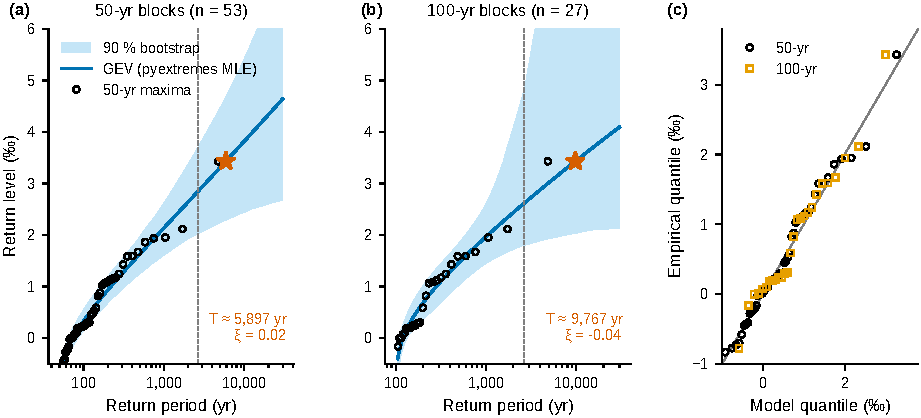
\includegraphics[width=\textwidth,height=0.50\textheight,keepaspectratio]{fig07_bm_gev}
  \par\vspace{-0.3em}
  \begin{itemize}\footnotesize\setlength{\itemsep}{1pt}
    \item \textbf{Reading the figure.} (a, b) How dry a block maximum is for
          each return period, with 50-yr and 100-yr blocks. Circles: observed
          maxima ($T_i$); blue line: fitted GEV; band: 90\,\% bootstrap
          range; star: 520--525 CE; dashed line: record length. (c) Observed
          versus model quantiles: points near the line mean a good fit.
    \item \textbf{Result.} The curve reaches the 520--525 CE value at about
          \alert{\nTFifty{} yr} (50-yr blocks) and \alert{\nTHundred{} yr}
          (100-yr blocks), well beyond the \nSpan-yr record.
  \end{itemize}
\end{frame}

% =================================================================== 16
\begin{frame}{Results in numbers}
  \centering\small
  \begin{tabular}{@{}lcc@{}}
    \toprule
    & 50-yr blocks & 100-yr blocks \\
    \midrule
    Number of maxima $m$ & \nNFifty & \nNHundred \\
    Location $\mu$ (\permil) & \nMuFifty & \nMuHundred \\
    Scale $\sigma$ (\permil) & \nSigmaFifty & \nSigmaHundred \\
    Shape $\xi$ (5--95\,\%) & \nXiFifty{} (\nXiLoFifty{} to \nXiHiFifty)
      & \nXiHundred{} (\nXiLoHundred{} to \nXiHiHundred) \\
    1,000-yr return level (\permil) & \nRLThousandFifty{}
      (\nRLThousandLoFifty--\nRLThousandHiFifty)
      & \nRLThousandHundred{} (\nRLThousandLoHundred--\nRLThousandHiHundred) \\
    Return period of 520--525 CE (yr) & \alert{\nTFifty} & \alert{\nTHundred} \\
    \quad bootstrap lower bound (5\,\%) & \nTBootLoFifty & \nTBootLoHundred \\
    Chance of such an event in \nSpan{} yr & \nPRecFifty\,\% & \nPRecHundred\,\% \\
    \bottomrule
  \end{tabular}
  \par\medskip
  \begin{itemize}\footnotesize\setlength{\itemsep}{2pt}
    \item $\xi$ is close to zero: the tail is nearly Gumbel, with no clear
          ceiling.
    \item The 520--525 CE value ($+\nEventLevel$\permil) lies far above
          the 1,000-yr return level (about 2\permil). Even the bootstrap
          lower bounds exceed 1,500 yr.
  \end{itemize}
\end{frame}

% =================================================================== 17
\begin{frame}{Check: removing the event from its own fit}
  \begin{columns}[c]
    \begin{column}{0.53\textwidth}\small
      \begin{itemize}\setlength{\itemsep}{3pt}
        \item The fitted curve includes the 520--525 CE value itself, which
              pulls the tail toward it and makes the event look
              \alert{less} rare.
        \item Analogy: judging whether a basketball player is unusually tall
              with an average that already includes that player.
        \item Test: remove 500--530 CE, refit the GEV, and ask how
              surprising the event is to the rest of the record.
      \end{itemize}
    \end{column}
    \begin{column}{0.43\textwidth}
      \begin{block}{Result without the event}
        \small
        \begin{tabular}{@{}lcc@{}}
          & 50-yr & 100-yr \\
          \midrule
          Shape $\xi$ & \nXiWithoutFifty & \nXiWithoutHundred \\
          $T$ (yr) & \nTWithoutFifty & \nTWithoutHundred \\
        \end{tabular}
        \par\smallskip
        The next driest value is only $+\nSecondPeak$\permil. Without the
        event, the tail acquires a ceiling: the event becomes \alert{about
        nine times rarer} (50-yr blocks) or lies \alert{beyond the ceiling}
        (100-yr blocks).
      \end{block}
    \end{column}
  \end{columns}
\end{frame}

% =================================================================== 18
\begin{frame}{Physical checks: the excursion is a real signal}
  \begin{itemize}\small\setlength{\itemsep}{4pt}
    \item \textbf{Not a single bad analysis.} \nNHighWindow{} of the
          \nNHighAll{} samples above $+2.5$\permil{} in the whole record lie
          between 515 and 535 CE, on separate growth layers about 2 mm
          apart.
    \item \textbf{Not temperature.} At about $-0.2$\permil{} per
          \textdegree C, the excursion would require a cave cooling of more
          than 15\,\textdegree C \citep{Lachniet2009}.
    \item \textbf{Independent indicators agree.} During the same interval
          the paper reports a narrower stalagmite (slower drips) and higher
          $\delta^{13}$C (less effective moisture)
          \citep{Fleitmann2022}.
    \item \textbf{Not only a dry century.} The smooth 300-yr trend was just
          $\nBgEvent$\permil{} at the time, close to today; the excursion
          rises far above it.
  \end{itemize}
  \par\medskip
  \small The excursion is a genuine hydroclimate signal. Its size in
  \permil{} is amplified by the processes on the previous slides.
\end{frame}

% =================================================================== 19
\begin{frame}{Physical drivers of the drought proposed by the paper}
  \begin{itemize}\small\setlength{\itemsep}{4pt}
    \item \textbf{Winter-spring rainfall.} Lake and cave records from Iran,
          the Levant and Lebanon dry out from about 480--510 CE, while a
          Turkish lake becomes wetter. This pattern suggests that storm
          tracks shifted north, so fewer Mediterranean fronts reached
          Arabia \citep{Fleitmann2022}.
    \item \textbf{Summer monsoon.} Northern Hemisphere summer insolation was
          near its Holocene minimum; monsoon records from Oman, the Arabian
          Sea, Ethiopia and India reach their weakest values in the sixth
          century \citep{Fleitmann2022}.
    \item \textbf{Timing of the Late Antique Little Ice Age.} The cooling
          began in 536 CE \citep{Buntgen2016}, after the H12 peak, so it
          cannot have triggered it, although it may have prolonged the
          stress.
    \item \textbf{Limit of this record.} H12 integrates winter-spring
          rainfall at one site; it cannot separate these drivers.
  \end{itemize}
\end{frame}

% =================================================================== 20
\begin{frame}{Historical context: consistent timing, limited precision}
  \centering
  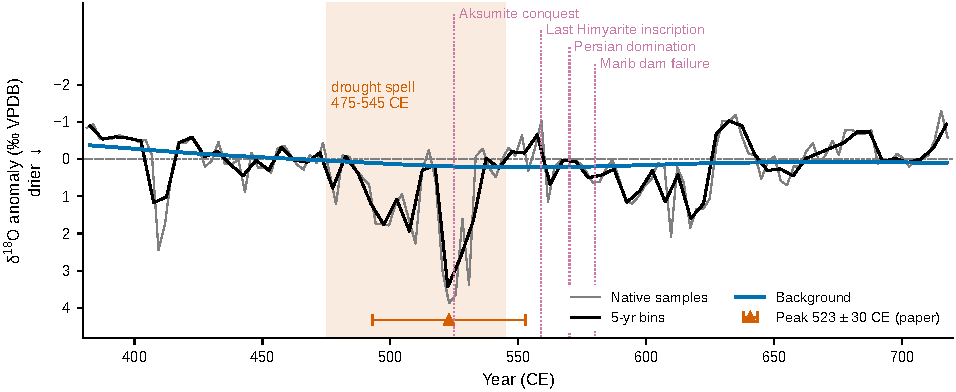
\includegraphics[width=\textwidth,height=0.50\textheight,keepaspectratio]{fig12_context}
  \par\vspace{-0.3em}
  \begin{itemize}\footnotesize\setlength{\itemsep}{1pt}
    \item \textbf{Reading the figure.} Drought plots downward; orange box:
          the 475--545 CE drought spell; orange bar: the peak age and its
          dating uncertainty; purple lines: historical events.
    \item The $\pm$30-yr age uncertainty of the peak covers the Aksumite
          conquest (525 CE) and approaches the last Himyarite inscription
          (about 559 CE).
    \item Any event of those decades would match equally well: the timing is
          \alert{consistent with} the historical sequence but cannot single
          it out.
  \end{itemize}
\end{frame}

% =================================================================== 21
\begin{frame}{What is robust and what is not}
  \centering\small
  \begin{tabular}{@{}p{0.33\textwidth}p{0.43\textwidth}p{0.14\textwidth}@{}}
    \toprule
    Claim & Evidence & Status \\
    \midrule
    A real excursion, not an error & Several growth layers; temperature
      cannot explain it & \textcolor{okgreen}{\textbf{Strong}} \\
    Driest value in 2,600 yr & Rank 1 of \nNBins{} values; \nZscore{}
      standard deviations & \textcolor{okgreen}{\textbf{Strong}} \\
    Return period far longer than the record & \nTFifty{} and \nTHundred{}
      yr; bootstrap lower bounds above 1,500 yr
      & \textcolor{okgreen}{\textbf{Strong}} \\
    A precise return period & Depends on block size and on whether the
      event is in the fit & \textcolor{okverm}{\textbf{Weak}} \\
    Causal link to Himyar's fall & Timing within $\pm$30 yr; no mechanism
      in this record & \textcolor{okverm}{\textbf{Weak}} \\
    \bottomrule
  \end{tabular}
\end{frame}

% =================================================================== 22
\begin{frame}{Caveats}
  \begin{itemize}\small\setlength{\itemsep}{3pt}
    \item \textbf{One archive and one proxy.} A single stalagmite stands in
          for southern Arabia, and only \dO{} is analyzed.
    \item \textbf{Proxy, not rainfall.} The amount effect and cave kinetics
          make \dO{} respond nonlinearly to rainfall, and the event lies far
          outside the modern calibration range. The return periods describe
          the proxy, not millimeters of rain.
    \item \textbf{Few maxima.} \nNFifty{} or \nNHundred{} block maxima
          constrain the tail only loosely, which is why the shape $\xi$ and
          the return period carry wide uncertainty.
    \item \textbf{Ages.} No age-model ensemble is published, so dating
          uncertainty is discussed but not propagated.
    \item \textbf{Data copy.} The table was transcribed from the NOAA
          archive; the code reads the original file automatically once it is
          placed in \texttt{data/raw}.
  \end{itemize}
\end{frame}

% =================================================================== 23
\begin{frame}{Conclusions}
  \begin{enumerate}\small\setlength{\itemsep}{3pt}
    \item The 520--525 CE excursion in H12 is a real hydroclimate signal and
          the \alert{driest value in 2,600 years}, \nZscore{} standard
          deviations above the rest of the record.
    \item The amount effect and cave kinetics both raise \dO{} in dry years,
          so the proxy amplifies the drought.
    \item Block maxima with a GEV curve give a return period of about
          \alert{\nTFifty{} to \nTHundred{} years}, far longer than the
          record; removing the event from the fit makes it rarer still.
    \item The exact number is uncertain, but the drought was exceptional on
          a multi-millennial scale. Its link to Himyar rests on timing that
          dating resolves only to a few decades.
  \end{enumerate}
  \par\smallskip
  \footnotesize\textbf{Reproducibility.} Code, data, figures and reports
  (MIT license): \url{https://github.com/sandyherho/utsCuacaIklimEks}.
  Running \texttt{python scripts/run\_all.py} reproduces every number in
  these slides.
\end{frame}

% =================================================================== 24
\begin{frame}{References}
  \renewcommand{\bibsection}{}
  \fontsize{6.2}{7.2}\selectfont
  \begin{multicols}{2}
    \bibliographystyle{abbrvnat}
    \bibliography{refs}
  \end{multicols}
\end{frame}

\end{document}
